\documentclass[12pt]{article}

%%%%%%%%%%%%%%%%
%%% General Packages %%%%
%%%%%%%%%%%%%%%%
\usepackage{amsmath,epsfig,amssymb,amsfonts,amsthm,epsfig,verbatim, titlesec}
\usepackage{color,xcolor,graphicx,lscape,longtable}
\usepackage{float}

%\usepackage{enumitem}
\usepackage{mathrsfs, tikz}
\usepackage{color}
\usepackage{graphicx}
\usepackage{multirow}
\usepackage{bm}
%\usepackage{beamerthemesplit}
\usepackage{amsmath,amssymb,latexsym,epsfig,graphics}
\usepackage{natbib,url}
\usepackage{caption, subcaption}
\usepackage{graphicx, color}
\definecolor{brickred}{rgb}{0.6,0,0}
\RequirePackage[backref=page]{hyperref} \hypersetup{
	colorlinks=true,       % false: boxed links; true: colored links
	linkcolor=magenta,          % color of internal links
	citecolor=blue,        % color of links to bibliography
	filecolor=magenta,      % color of file links
	urlcolor=brickred           % color of external links
}
%\usepackage[all]{xy}
\usepackage{booktabs}
\usepackage{multirow}

\usepackage[ruled]{algorithm2e}

%%%%%%%%%%%%%%%%
%%%% Page Settings %%%%%
%%%%%%%%%%%%%%%%
\newcommand{\indep}{\;\, \rule[0em]{.03em}{.67em} \hspace{-.25em}
\rule[0em]{.65em}{.03em} \hspace{-.25em}\rule[0em]{.03em}{.67em}\;\,}
\setlength{\textheight}{8.2in} \setlength{\textwidth}{7.1in}
\setlength{\topmargin}{-0pt} \setlength{\oddsidemargin}{-0.3in}
\setlength{\evensidemargin}{0pt} \tolerance=500
%\setlength{\textheight}{8.2in} \setlength{\textwidth}{6.5in}
%\setlength{\topmargin}{-0pt} \setlength{\oddsidemargin}{0pt}
%\setlength{\evensidemargin}{0pt} \tolerance=500

\tolerance=500

%\titlespacing\section{0pt}{5pt}{0pt}
%\titlespacing\subsection{0pt}{5pt}{0pt}

\newcommand{\Appendix}{\appendix
	\def\thesection{Appendix~\Alph{section}}
	\def\thesubsection{\Alph{section}.\arabic{subsection}}}

%%%%%%%%%%%%%%%
%%%%% Macros: %%%%%%
%%%%%%%%%%%%%%%

\newcommand{\Ex}{\mathbb{E}}
\def\rmd{\,\mathrm{d}}
\def\dist{\mathrm{dist}}
\def\bI{\mathbb{I}}
\def\sf{\mathscr{F}}
\def\cH{\mathscr{H}}
\renewcommand{\thealgocf}{\Roman{algocf}}
\newcommand{\argmin}{\ensuremath{\operatornamewithlimits{arg\,min}}}
\newcommand{\argmax}{\ensuremath{\operatornamewithlimits{arg\,max}}}
\def\trans{^{\top}}
\def\indi{\mathbf{I}}

\def\wh{\widehat}
\def\wt{\widetilde}

\def\normal{\mathcal{N}}
\def\pr{\mathrm{pr}}
\def\logit{\mathrm{logit}}
\def\rest{\mathrm{rest}}
\def\vec{\mathrm{vec}}
\def\cov{\mathrm{cov}}
\def\var{\mathrm{var}}
\def\Dirichlet{\mathrm{Dirichlet}}
\def\corr{\mathrm{corr}}
\def\tr{\mathrm{tr}}
\def\sumi{\sum_{i=1}^n}
\def\diag{\mathrm{diag}}
\def\AIC{\mathrm{AIC}}
\def\BIC{\mathrm{BIC}}
\def\diag{\mathrm{diag}}
\def\bias{\mathrm{bias}}\def\povr{\buildrel p\over\longrightarrow}

\def\naive{\mathrm{naive}}
\def\refhg{\hangindent=20pt\hangafter=1}
\def\refmark{\par\vskip -1mm\noindent\refhg}
\def\ccdot{{\bullet}}

\def\myZ{{\bf Z}}
\def\myalpha{{\cal A}}

\newcommand{\uA}       {\bm{A}}
\newcommand{\ua}       {\bm{a}}
\newcommand{\uB}       {\bm{B}}
\newcommand{\ub}       {\bm{b}}
\newcommand{\uC}       {\bm{C}}
\newcommand{\uc}       {\bm{c}}
\newcommand{\uD}       {\bm{D}}
\newcommand{\ud}       {\bm{d}}
\newcommand{\uE}       {\bm{E}}
\newcommand{\ue}       {\bm{e}}
\newcommand{\uF}       {\bm{F}}
\newcommand{\uf}       {\bm{f}}
\newcommand{\uG}       {\bm{G}}
\newcommand{\ug}       {\bm{g}}

\newcommand{\uH}       {\bm{H}}
\newcommand{\uh}       {\bm{h}}
\newcommand{\uI}       {\bm{I}}
\newcommand{\ui}       {\bm{i}}
\newcommand{\uJ}       {\bm{J}}
\newcommand{\uj}       {\bm{j}}
\newcommand{\uK}       {\bm{K}}
\newcommand{\uk}       {\bm{k}}
\newcommand{\uL}       {\bm{L}}
\newcommand{\ul}       {\bm{l}}
\newcommand{\uM}       {\bm{M}}
\newcommand{\um}       {\bm{m}}
\newcommand{\uN}       {\bm{N}}
\newcommand{\un}       {\bm{n}}
\newcommand{\uO}       {\bm{O}}
\newcommand{\uP}       {\bm{P}}
\newcommand{\up}       {\bm{p}}
\newcommand{\uQ}       {\bm{Q}}
\newcommand{\uq}       {\bm{q}}
\newcommand{\uR}       {\bm{R}}
\newcommand{\ur}       {\bm{r}}
\newcommand{\uS}       {\bm{S}}
\newcommand{\us}       {\bm{s}}
\newcommand{\uT}       {\bm{T}}
\newcommand{\ut}       {\bm{t}}
\newcommand{\uU}       {\bm{U}}
\newcommand{\uu}       {\bm{u}}
\newcommand{\uV}       {\bm{V}}
\newcommand{\uv}       {\bm{v}}
\newcommand{\uW}       {\bm{W}}
\newcommand{\uw}       {\bm{w}}
\newcommand{\uX}       {\bm{X}}
\newcommand{\ux}       {\bm{x}}
\newcommand{\uY}       {\bm{Y}}
\newcommand{\uy}       {\bm{y}}
\newcommand{\uZ}       {\bm{Z}}
\newcommand{\uz}       {\bm{z}}

\newcommand{\ualpha}            {\bm{\alpha}}
\newcommand{\ubeta}             {\bm{\beta}}
\newcommand{\ugamma}            {\bm{\gamma}}
\newcommand{\udelta}            {\bm{\delta}}
\newcommand{\uepsilon}          {\bm{\epsilon}}
\newcommand{\uvarepsilon}       {\bm{\varepsilon}}
\newcommand{\uzeta}             {\bm{\zeta}}
\newcommand{\ueta}              {\bm{\eta}}
\newcommand{\utheta}            {\bm{\theta}}
\newcommand{\uvartheta}         {\bm{\vartheta}}
\newcommand{\uiota}             {\bm{\uiota}}
\newcommand{\ukappa}            {\bm{\kappa}}
\newcommand{\ulambda}           {\bm{\lambda}}
\newcommand{\umu}               {\bm{\mu}}
\newcommand{\unu}               {\bm{\nu}}
\newcommand{\uxi}               {\bm{\xi}}
\newcommand{\uo}                {\bm{\o}}
\newcommand{\upi}               {\bm{\pi}}
\newcommand{\uvarpi}            {\bm{\varpi}}
\newcommand{\urho}              {\bm{\rho}}
\newcommand{\uvarrho}           {\bm{\varrho}}
\newcommand{\usigma}            {\bm{\sigma}}
\newcommand{\uvarsigma}         {\bm{\varsigma}}
\newcommand{\utau}              {\bm{\tau}}
\newcommand{\uupsilon}          {\bm{\upsilon}}
\newcommand{\uphi}              {\bm{\phi}}
\newcommand{\uvarphi}           {\bm{\varphi}}
\newcommand{\uchi}              {\bm{\chi}}
\newcommand{\upsi}              {\bm{\psi}}
\newcommand{\uomega}            {\bm{\omega}}

\newcommand{\uGamma}            {\bm{\Gamma}}
\newcommand{\uDelta}            {\bm{\Delta}}
\newcommand{\uTheta}            {\bm{\Theta}}
\newcommand{\uLambda}           {\bm{\Lambda}}
\newcommand{\uXi}               {\bm{\Xi}}
\newcommand{\uPi}                {\bm{\Pi}}
\newcommand{\uSigma}            {\bm{\Sigma}}
\newcommand{\uUpsilon}          {\bm{\Upsilon}}
\newcommand{\uPhi}              {\bm{\Phi}}
\newcommand{\uPsi}              {\bm{\Psi}}
\newcommand{\uOmega}            {\bm{\Omega}}

\newcommand{\uzero}            {\bm{0}}
\newcommand{\uone}               {\bm{1}}

\newcommand{\mti}      {\mbox{$\mathcal{I}$}}

\newcommand{\mm}      {\mbox{$\mathcal{M}$}}

\newcommand{\Trans}  {\mathrm{T}}

\newcommand{\Px}  {\mathbb{P}}
\newcommand{\RedText} {\textcolor[rgb]{1,0,0}}
%%%%%%%%%%%%%%
%%% Theorems %%%%%%
%%%%%%%%%%%%%%
%\newcommand{\qed}{\hfill\hfill\vbox{\hrule\hbox{\vrule\squarebox
\newtheorem{Th}{\underline{\bf Theorem}}
\newtheorem{Proof}{Proof}
\newtheorem{Mth}{Main Theorem}
\newtheorem{Def}{Definition}
\newtheorem{Rem}{\underline{\bf Remark}}
\newtheorem{Qes}{Question}
\newtheorem{proposition}{Proposition}
\newtheorem{Lem}{\underline{\bf Lemma}}
\newtheorem{Cor}{\underline{\bf Corollary}}
\newtheorem{Exa}{Example}
%\newtheorem{Eq}{Equation}


%%%%%%%%%%%%%
%%% Comments %%%%
%%%%%%%%%%%%%
\def\boxit#1{\vbox{\hrule\hbox{\vrule\kern6pt
			\vbox{\kern6pt#1\kern6pt}\kern6pt\vrule}\hrule}}
\def\kejuncomment#1{\vskip 2mm\boxit{\vskip 2mm{\color{cyan}\bf#1} {\color{cyan}\bf -- Kejun\vskip 2mm}}\vskip 2mm}
\definecolor{smgreen}{rgb}{0.3,0.7,0.3}
\newcommand{\kejun}[1]{{\bf\textcolor{smgreen}{[Kejun: #1]}}}
%\newcommand{\kejun}[1]{{\bf\textcolor{cyan}{[Kejun: #1]}}}
\newcommand{\kejunadd}[1]{{\bf\textcolor{red}{#1}}}


\begin{document}
	
\baselineskip=24pt
\allowdisplaybreaks
\title{The Cure Model for Teeth Data}
\date{}
\author{Fengyu Zhang}
\maketitle

\section{Introduction \label{sec:intro}}
In survival analysis, one usually assumes that all subjects under study will eventually experience the event of interest. However, there are various situations for which this assumption is not realistic. For instance, when the event of interest is the time until a patient progresses or relapses from a certain disease, then patients who are cured from the disease will never experience the event. Those observations will be considered as “long-term survivors” or as “cured,” and their survival time will be set to infinity. Cure models are survival models that have been developed to take this feature into account.

When information on covariates is present, a commonly used cure
regression model is the mixture cure model. It assumes that the survival
function \(S(t|x,z) = P(T>t|X=x,Z=z)\) of survival time \(T\) given a
set of covariates \((X^t,Z^t)\) is given by
\[S(t|x,z) = 1-p(x)+p(x)S_u(t|z),\qquad t\geqslant 0,\] where
\(p(x)=P(B=1|X=x)\) is the conditional probability of being uncured
(often referred to as the `incidence') with \(B=I(T<\infty)\) the latent
uncured status; and \(S_u(t|z)=P(T>t|B=1,Z=z)\) is the conditional
survival function for the uncured subjects (often referred to as the
`latency'). Amico et al.(2018) proposed a single-index model for
\(p(x)\) to allow the cure rate to be more flexible, i.e., there exists
an unknown link function \(g(\cdot)\) such that
\[p(x)=g(\gamma^\mathrm{T}x).\] The link function can be any (smooth)
function with values between 0 and 1, and will be estimated
nonparametrically using kernel methods.

For the part of latency, we consider a Cox propotional hazards (PH)
model (Cox 1972) with the following form
\[S_u(t|z) = S_0(t)^{\exp(\beta^T z)},\] where \(S_0(t)=P(T>t|B=1)\) is
the baseline conditional survival function. The conditional hazard
function is given by \(\lambda_u(t|z) = \lambda_0(t)\exp(\beta^T z),\)
where \(\lambda_0(t)\) is the baseline conditional hazard function.

In the survival analysis, we usually observe the couple \((Y,\delta)\)
instead of the survival time \(T\), where
\(Y = \min(T,C),\delta = I(T\leqslant C)\). Let
\((Y_i,\delta_i,X_i,Z_i),i=1\ldots,n\) be i.i.d. observations. Assuming
non-informative censoring, the likelihood of an observation
\((y,\delta,x,z)\) is given by
\[L(y,\delta,x,z) = \{g(\gamma^Tx)f_u(y|z)\}^\delta\{1-g(\gamma^Tx)S_u(y|z)\}^{1-\delta},\]
where \(f_u(t|z) = -\frac{d}{dt}S_u(t|z).\)

\section{Dataset}

\subsection{Overview}
The data is about a kind of dental disease. The dataset contains 65890 observations of 20 variables. In order to be operable, we select the observations with “tooth=2” which is a molar and rename some of the columns for convenience. Also, we remove some irrelevant variables. Figure \ref{fig:data_overview} and \ref{fig:select} show a overview of the dataset and the covariates we select, respectively. Besides age and gender, we have chosen four numeric covariates and some category variables. Table \ref{tab:covar} gives some of the explanations of the covariates we are interested. Covariates that are not shown in the table are binary variables.
\begin{figure}[H]
	\begin{subfigure}{1\textwidth}
		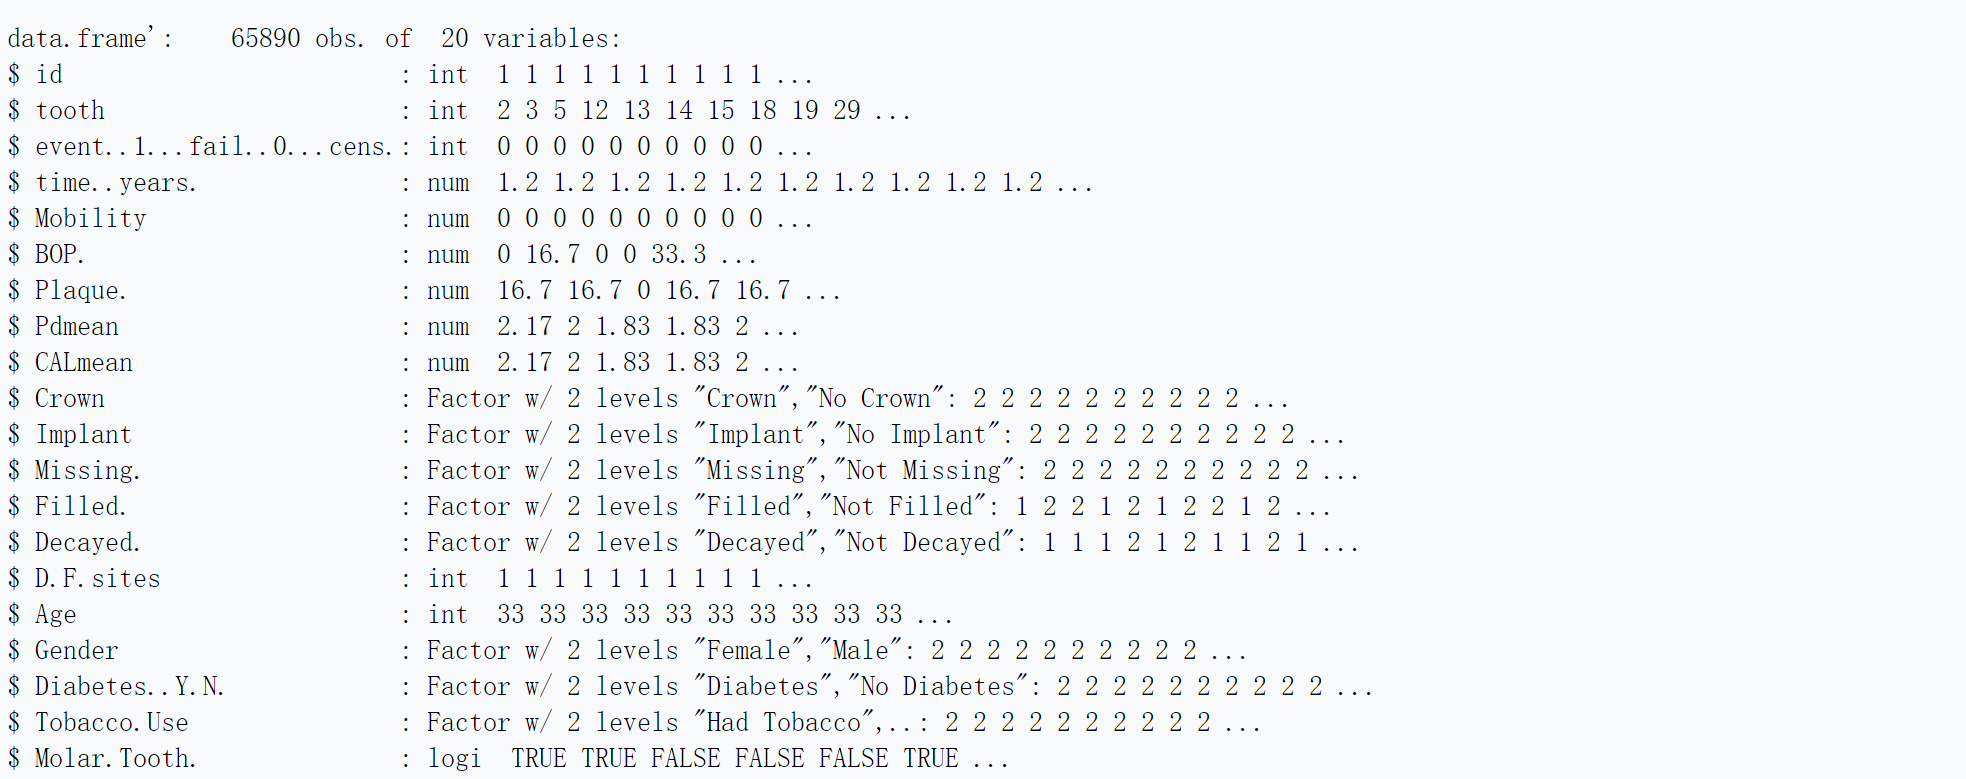
\includegraphics[width=1\textwidth]{figure/data_overview}
		\subcaption{Data Overview}\label{fig:data_overview}
	\end{subfigure}
	\begin{subfigure}{1\textwidth}
		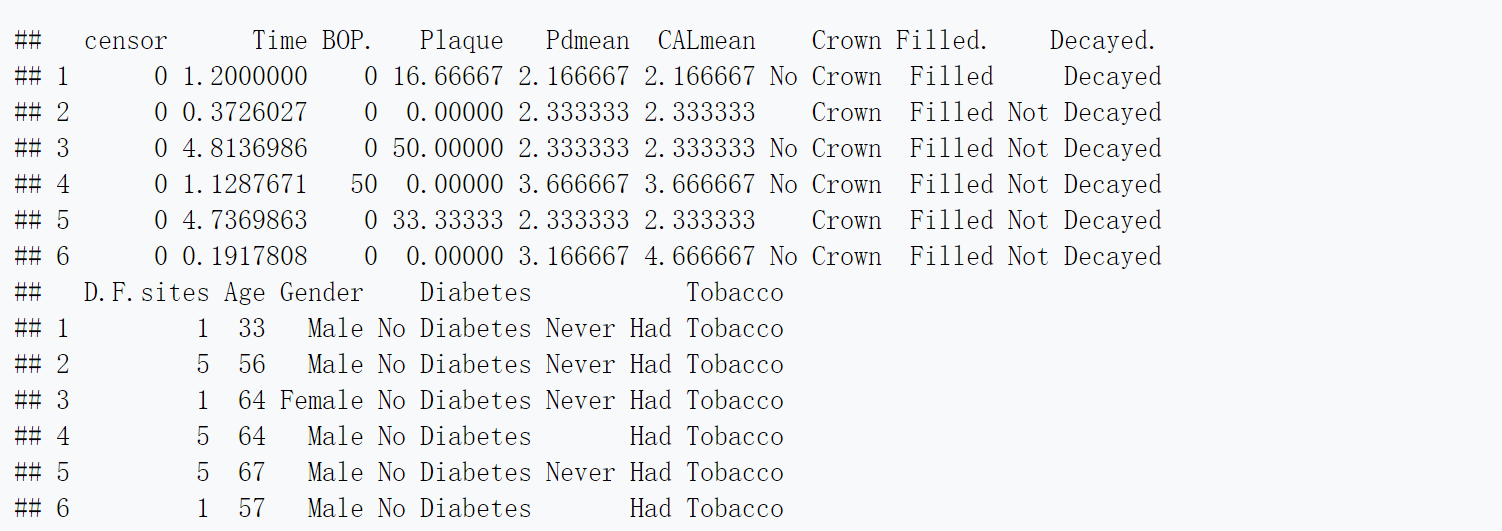
\includegraphics[width=1\textwidth]{figure/preprocess}
		\subcaption{Data pre-selection}\label{fig:select}
	\end{subfigure}
\end{figure}



\begin{table}[H]
	\centering
	\begin{tabular}{cc}
		Covariate & Explanation\\
		\hline
		BOP\%:  & \% of tooth-sites that bled when probed \\
		Plaque\%:  & \% of tooth-sites stained with bacterial plaque \\
		Pdmean:  & mean pocket depth for that tooth \\
		CALmean:  & mean clinical attachment level for that tooth \\
		\hline
	\end{tabular}%
	\caption{}\label{tab:covar}%
\end{table}%

\subsection{Exploratory Data Analysis}

\begin{figure}[H]
	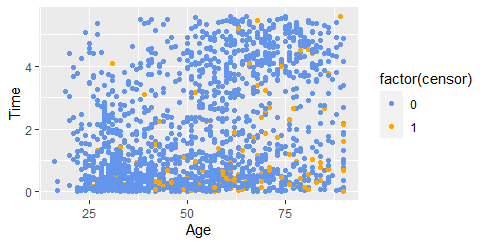
\includegraphics[width=1\textwidth]{figure/censor1}
	\caption{Censor rate}\label{fig:censor}
\end{figure}
Figure \ref{fig:censor} dipects the censor rate of the data. Each point represents an observation and the 92\% of the observations are censored. We can see that the censor rate is high and a cure model seems therefore appropriate for these data.

Figure \ref{fig:4fig} displays the relationship between two of the numeric covariates and age together with gender.
\begin{figure}[H]
	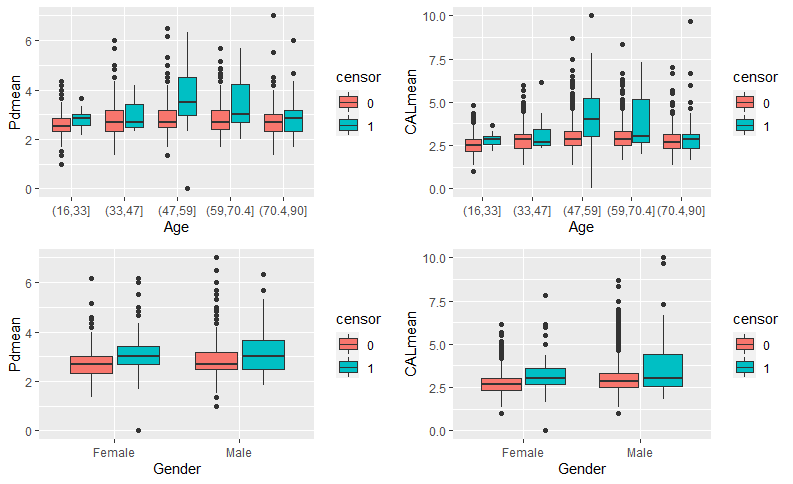
\includegraphics[width=1\textwidth]{figure/4fig}
	\caption{}\label{fig:4fig}
\end{figure}

\section{Model and Estimation}
\subsection{Model Assumption}
\cite{Boag1949} and \cite{Farewell1982} originally proposed a mixture cure model which assumes that the survival function has the following form:
\begin{equation}\label{equ:sur_fun}
S(t|x,z) = P(T>t|x,z) = 1 - p(x) + p(x)S_u(t|z),\quad t\geqslant 0,
\end{equation}
where 
\begin{itemize}
	\item 	$p(x)=\Px(B=1|X=x)$ is the conditional probability of being uncured (often referred to as the '{incidence}') with $B=I(T<\infty)$ the latent uncured status.
	\item $S_u(t|z)=\Px(T>t|B=1,Z=z)$ is the conditional survival function for the uncured subjects (often referred to as the '{latency}')
\end{itemize}
Here, the covariate vectors $X$ and $Z$ can contain (partially) the same covariates, but they can also be completely different.

For the part of latency ($S_u(t|z)$), we consider a Cox propotional hazards (PH) model (\citealt{Cox1972}) with the following form 
\begin{equation}
S_u(t|z) = S_0(t)^{\exp(\beta^\Trans z)}
\end{equation}
where $S_0(t)=\Px(T>t|B=1)$ is the baseline conditional survival function. The conditional hazard function is given by 
$$\lambda_u(t|z)=\lambda_0(t)\exp(\beta^\Trans z),$$
where $\lambda_0(t)$ is the baseline hazard function.
For the part of incidence (uncured rate $p(x)$), two models are considered. 
\begin{enumerate}
	\item Logistic model (common assumption): $$p(x)=\frac{\exp(\gamma_0+\gamma^\Trans x)}{1+\exp(\gamma_0+\gamma^\Trans x)}$$
	for some parameter vector $\gamma$ and an intercept $\gamma_0$. The logistic model is easy to interpret and estimate                                                                                                                                                                                                                                                                                                                                                                                                                                                        
	\item Single-index model:
	$$p(x) = g(\gamma^\Trans x)$$
	for any smooth link function $g$ with values between 0 and 1. The single-index model has nonparametric link function and therefore much more flexibel than the logistic model. Besides, it does not suffer from the curse-of-dimensionality problems.
\end{enumerate}

\subsection{Maximum Likelihood Estimator}

	In survival analysis, we usually observe the couple $(Y,\delta)$ instead of the survival time $T$, where $Y=\min (T,C), \delta = I(T\leqslant C)$, and $C$ is the censoring time. As often, we assume $T$ and $C$ are independent given the covariates $X,Z$. 

Denote $(Y_i,\delta_i,X_i,Z_i),i=1,\ldots,n$ be i.i.d. realizations of $(Y,\delta,X,Z)$, the likelihood function takes the form
\begin{equation}\label{equ:L_c}
L = \prod_{i=1}^{n}\{p(X_i)f_u(Y_i|Z_i)\}^{\delta_i}\cdot \left[\{1-p(X_i)\}+p(X_i)S_u(Y_i|Z_i)\right]^{1-\delta_i}.
\end{equation}
where $f_u(t|z) = -(d/dt)S_u(t|z)$ is the conditional density function. The likelihood has two types of contributions: from censored and from the uncensored observations. 

We use EM algorithm to handle the fact that the cure status $B_i$ is unobserved. The complete-data likelihood is given by
\begin{equation}\label{equ:com_data}
\begin{aligned}
L_c =& \prod_{i=1}^{n}\{p(X_i)\lambda_u(Y_i|Z_i)S_u(Y_i|Z_i)\}^{B_i \delta_i}\times \\ &\left[\{1-p(X_i)\}^{1-B_i}+\{p(X_i)S_u(Y_i|Z_i)\}^{B_i} \right]^{1-\delta_i}
\end{aligned}
\end{equation}
Then we need to calculate the conditional expectation of the log-likelihood given the observed data and the current parameter values. As the log-likelihood is linear in $B$, it is the same as computing $$\Ex(B_i|\mathcal{O},\Theta^{(m-1)}) := W_i^{(m)},$$
where $\mathcal{O} = \{(Y_i,\delta_i,X_i,Z_i),i=1,\ldots,n\}$ are observed data and $ \Theta = (\gamma,\beta,S_0)$ for logistic model and $\Theta = (\gamma,\beta,S_0,g)$ for single-index model.

In M-step, we maximize the expected log-likelihood which is obtained by replacing $B_i$ by $W_i^{(m)}$ in the equation (\ref{equ:com_data}):
\begin{equation}
\begin{aligned}
\tilde{L}_c=& \prod_{i=1}^{n}\{p(X_i)\lambda_u(Y_i|Z_i)S_u(Y_i|Z_i)\}^{W_i^{(m)} \delta_i}\times \\ 
&\left[\{1-p(X_i)\}^{1-W_i^{(m)}}+\{p(X_i)S_u(Y_i|Z_i)\}^{W_i^{(m)}} \right]^{1-\delta_i}.
\end{aligned}
\end{equation}
After some algebra, $\tilde{L}_c$ can be written as the product of two parts:
\begin{equation}
\begin{aligned}
\tilde{L}_c &= \prod_{i=1}^n \left[p(X_i)^{W_i^{(m)}}\{1-p(X_i)\}^{1-W_i^{(m)}}\right]\times 
\prod_{i=1}^n \{\lambda_u(Y_i|Z_i)^{\delta_i}S_u(Y_i|Z_i)\}^{W_i^{(m)}} \\
&= \tilde{L}_1 \times \tilde{L}_2.
\end{aligned}
\end{equation}
It can be maximized separately for the two parts of the model.

\subsection{Estimators of Incidence and Latency}
Although the framework of the EM algotirhm is constructed, one problem is that how to estimate the parameters when we use the single-index model in the incidence part. \cite{Ich1993} proposed a leave-one-out kernel estimator of $g(\gamma^\Trans X_i)$:
$$\sum_{j \neq i}^{n} \frac{K\left(\frac{\gamma^{t} X_{i}-\gamma^{t} X_{j}}{h}\right)}{\sum_{l \neq i}^{n} K\left(\frac{\gamma^{t} X_{i}-\gamma^{t} X_{l}}{h}\right)} B_{j}.$$
We need to replace $B_j$ by $W_j^{(m)}$ obtained in the E-step and then the estimator becomes
\begin{equation}\label{equ:ker_est}
\tilde{g}_{-i}^{(m)}\left(\gamma^{t} {X}_{i}\right)=\sum_{j \neq i}^{n} \frac{K\left(\frac{\gamma^{t} X_{i}-\gamma^{t} X_{j}}{h}\right)}{\sum_{l \neq i}^{n} K\left(\frac{\gamma^{t} X_{i}-\gamma^{t} X_{l}}{h}\right)} W_{j}^{(m)}
\end{equation}
The kernel estimator (\ref{equ:ker_est}) is substitued in $\tilde{L}_1$, and $\gamma$ is estimated by maximizing the likelihood.

As for the latency ($\tilde{L}_2$), note that 
$\tilde{L}_2=\prod_{i=1}^{n}\left[\left\{\lambda_{0}\left(Y_{i}\right) \exp \left(\boldsymbol{\beta}^{t} \boldsymbol{Z}_{i}\right)\right\}^{\delta_{i}} \exp \left\{-\Lambda_{0}\left(Y_{i}\right) \exp \left(\boldsymbol{\beta}^{t} \boldsymbol{Z}_{i}\right)\right\}\right]^{W_{i}^{(m)}}.$\\
\cite{Sy2000} propose a profile likelihood approach to estimate $\beta$.\\
First, given a fixed $\beta$, $\Lambda_{0}$ is estimated nonparametrically by 
\begin{equation}\label{equ:Lambda}
\sum_{j: Y_{(j)} \leq t} \frac{D_{j}}{\sum_{k \in R_{j}} W_{k}^{(m)} \exp \left(\boldsymbol{\beta}^{t} {Z}_{k}\right)},
\end{equation}
where $Y_{(j)}$ are order statitics, $D_j$ is the number of events at time $Y_{(j)}$ and $R_j$ is the risk set before $Y_{(j)}$.
Second, we plug (\ref{equ:Lambda}) in $\tilde{L}_2$, obtaining the partial likelihood
\begin{equation}\label{equ:L2}
\breve{\mathrm{L}}_{2}=\prod_{i=1}^{n}\left\{\frac{\exp \left({\beta}^{t} {Z}_{i}\right)}{\sum_{k \in R_{i}} W_{k}^{(m)} \exp \left({\beta}^{t} {Z}_{k}\right)}\right\}^{\Delta_{i}}
\end{equation}
The MLE of $\beta$ denoted by $\hat{\beta}^{(m)}$ is obtained by maximizing (\ref{equ:L2}). Then we plug $\hat{\beta}^{(m)}$ in (\ref{equ:Lambda}) to obtain $\hat{\Lambda}_0^{(m)}(t)$. We do alternative iterations until convergence.

\section{Result and Discussion}
Applying the two models above (SIC for single-index/cure model and LC for logistic/cure model) to the dataset and using Bootstrap method to compute the standard error of each estimator. Moreover, we test the significance of the covariates via Wald's test. The results are as following:
\begin{table}[htbp]
	\centering
	%\small
	\begin{tabular}{lrrrrrr}
		\hline
		& \multicolumn{3}{c}{SIC cure model} & \multicolumn{3}{c}{LC cure model} \\
		\hline
		Incidence & \multicolumn{1}{l}{Estimate} & \multicolumn{1}{l}{Std.error} & \multicolumn{1}{l}{p-value} & \multicolumn{1}{l}{Estimate} & \multicolumn{1}{l}{Std.error} & \multicolumn{1}{l}{p-value} \\
		\hline
		(intercept) & \multicolumn{1}{c}{-} & \multicolumn{1}{c}{-} & \multicolumn{1}{c}{-} & -4.54406 & 1.573907 & 0.003888 \\
		Age     & 0.56649 & 0.180257 & \RedText{0.0016741} & 0.031461 & 0.016599 & 0.058042 \\
		Gender  & -0.05871 & 0.346062 & 0.8652774 & -0.01342 & 0.55367 & 0.980664 \\
		BOP     & 0.6242  & 0.294932 & \RedText{0.0343093} & 1.692404 & 0.834437 & \RedText{0.04254} \\
		Plaque  & -0.4325 & 0.269344 & 0.1083279 & -0.00462 & 0.815525 & 0.995481 \\
		Pdmean  & -0.08126 & 0.244503 & 0.7396307 & 0.152681 & 0.281289 & 0.587275 \\
		CALmean & 0.303903 & 0.198951 & 0.12663 & 0.201554 & 0.165835 & 0.224218 \\
		&         &         &         &         &         &  \\
		\hline
		latency & \multicolumn{1}{l}{Estimate} & \multicolumn{1}{l}{Std.error} &
		\multicolumn{1}{l}{p-value} & \multicolumn{1}{l}{Estimate} & \multicolumn{1}{l}{Std.error} & \multicolumn{1}{l}{p-value} \\
		\hline
		Age     & -0.02421 & 0.010842 & \RedText{0.0255254} & -0.02177 & 0.016181 & 0.178525 \\
		Gender  & 0.148134 & 0.220341 & 0.5013959 & 0.193319 & 0.572714 & 0.735703 \\
		BOP     & 0.815028 & 0.426396 & 0.055949 & -0.29098 & 0.593112 & 0.623712 \\
		Plaque  & -0.77723 & 0.392359 & 0.0476001 & -0.68691 & 0.794442 & 0.387237 \\
		Pdmean  & 0.258177 & 0.160801 & 0.1083693 & -0.02163 & 0.224441 & 0.923235 \\
		CALmean & 0.343105 & 0.119735 & \RedText{0.0041631} & 0.359877 & 0.162896 & \RedText{0.027157} \\
		\hline
	\end{tabular}%
	\caption{Parameter Estimations, Std.error and Wald's test}
	\label{tab:result}
\end{table}%

\begin{itemize}
	\item According to the table, for the latency part, the effects for age, gender, Plaque and CALmean have the same direction and the estimates are very close. Only CALmean affects significantly the survivial time of uncured subjects in both of the two models.
	\item For the incidence part, we compare the predicted error of the incidence. First we divided the dataset into a training and test subsut, following 2/3-1/3 recommendations of \cite{Hastie2009}. We use the training set to estimate the parameters and calculate the prediction error which is given by
	\begin{equation}\label{equ:PE}
	PE =-\sum_{j=1}^{n_{test}} \log \left[\hat{p}\left({x}_{j}^{\text {test}}\right)^{\hat{w}_{j}}\left\{1-\hat{p}\left({x}_{j}^{\text {test}}\right)\right\}^{1-\hat{w}_{j}}\right]
	\end{equation}
	After computing, the prediction error for the SIC model equals to 57.65, while it is equal to 70.93 for the LC model, which means that the SIC model performs better in predicting the uncured status.
\end{itemize}


\newpage
\bibliographystyle{jasa}
\bibliography{Report.bib}

%#'''End loop'''.
%</div>

\end{document}